% Standalone TikZ figure: a 4x4 grid of fragments, with adjacency edges
% highlighted, used to illustrate how training labels are constructed.
%
% Include in another document with:
%     % Standalone TikZ figure: a 4x4 grid of fragments, with adjacency edges
% highlighted, used to illustrate how training labels are constructed.
%
% Include in another document with:
%     % Standalone TikZ figure: a 4x4 grid of fragments, with adjacency edges
% highlighted, used to illustrate how training labels are constructed.
%
% Include in another document with:
%     % Standalone TikZ figure: a 4x4 grid of fragments, with adjacency edges
% highlighted, used to illustrate how training labels are constructed.
%
% Include in another document with:
%     \input{fig_grid_labels.tex}
%
% Requires the host document to load \usepackage{tikz}. Compile
% fig_grid_labels_standalone.tex to preview.

\begin{tikzpicture}[
    cell/.style    = {draw=black!60, fill=blue!10, minimum size=11mm,
                      inner sep=0pt, font=\small},
    edge/.style    = {color=red!70!black, line width=1pt},
]

% --- 4x4 grid of cells ---
\foreach \r in {0,1,2,3}{
    \foreach \c in {0,1,2,3}{
        \pgfmathtruncatemacro{\idx}{\r*4 + \c}
        \node[cell] (n\r\c) at (\c*1.2, -\r*1.2) {$f_{\idx}$};
    }
}

% --- horizontal adjacency edges ---
\foreach \r in {0,1,2,3}{
    \foreach \c in {0,1,2}{
        \pgfmathtruncatemacro{\cnext}{\c+1}
        \draw[edge] (n\r\c) -- (n\r\cnext);
    }
}

% --- vertical adjacency edges ---
\foreach \c in {0,1,2,3}{
    \foreach \r in {0,1,2}{
        \pgfmathtruncatemacro{\rnext}{\r+1}
        \draw[edge] (n\r\c) -- (n\rnext\c);
    }
}

% --- legend ---
\node[anchor=west, font=\footnotesize] at (4.6, 0)
    {\textbf{$y_{ij} = 1$:} $f_i$ and $f_j$ adjacent (red edge)};
\node[anchor=west, font=\footnotesize] at (4.6, -0.6)
    {\textbf{$y_{ij} = 0$:} all other pairs};
\node[anchor=west, font=\footnotesize] at (4.6, -1.4)
    {16 fragments per image};
\node[anchor=west, font=\footnotesize] at (4.6, -2.0)
    {$4 \cdot 3 + 3 \cdot 4 = 24$ adjacent pairs};
\node[anchor=west, font=\footnotesize] at (4.6, -2.6)
    {$\binom{16}{2} - 24 = 96$ non-adjacent same-image pairs};

\end{tikzpicture}

%
% Requires the host document to load \usepackage{tikz}. Compile
% fig_grid_labels_standalone.tex to preview.

\begin{tikzpicture}[
    cell/.style    = {draw=black!60, fill=blue!10, minimum size=11mm,
                      inner sep=0pt, font=\small},
    edge/.style    = {color=red!70!black, line width=1pt},
]

% --- 4x4 grid of cells ---
\foreach \r in {0,1,2,3}{
    \foreach \c in {0,1,2,3}{
        \pgfmathtruncatemacro{\idx}{\r*4 + \c}
        \node[cell] (n\r\c) at (\c*1.2, -\r*1.2) {$f_{\idx}$};
    }
}

% --- horizontal adjacency edges ---
\foreach \r in {0,1,2,3}{
    \foreach \c in {0,1,2}{
        \pgfmathtruncatemacro{\cnext}{\c+1}
        \draw[edge] (n\r\c) -- (n\r\cnext);
    }
}

% --- vertical adjacency edges ---
\foreach \c in {0,1,2,3}{
    \foreach \r in {0,1,2}{
        \pgfmathtruncatemacro{\rnext}{\r+1}
        \draw[edge] (n\r\c) -- (n\rnext\c);
    }
}

% --- legend ---
\node[anchor=west, font=\footnotesize] at (4.6, 0)
    {\textbf{$y_{ij} = 1$:} $f_i$ and $f_j$ adjacent (red edge)};
\node[anchor=west, font=\footnotesize] at (4.6, -0.6)
    {\textbf{$y_{ij} = 0$:} all other pairs};
\node[anchor=west, font=\footnotesize] at (4.6, -1.4)
    {16 fragments per image};
\node[anchor=west, font=\footnotesize] at (4.6, -2.0)
    {$4 \cdot 3 + 3 \cdot 4 = 24$ adjacent pairs};
\node[anchor=west, font=\footnotesize] at (4.6, -2.6)
    {$\binom{16}{2} - 24 = 96$ non-adjacent same-image pairs};

\end{tikzpicture}

%
% Requires the host document to load \usepackage{tikz}. Compile
% fig_grid_labels_standalone.tex to preview.

\begin{tikzpicture}[
    cell/.style    = {draw=black!60, fill=blue!10, minimum size=11mm,
                      inner sep=0pt, font=\small},
    edge/.style    = {color=red!70!black, line width=1pt},
]

% --- 4x4 grid of cells ---
\foreach \r in {0,1,2,3}{
    \foreach \c in {0,1,2,3}{
        \pgfmathtruncatemacro{\idx}{\r*4 + \c}
        \node[cell] (n\r\c) at (\c*1.2, -\r*1.2) {$f_{\idx}$};
    }
}

% --- horizontal adjacency edges ---
\foreach \r in {0,1,2,3}{
    \foreach \c in {0,1,2}{
        \pgfmathtruncatemacro{\cnext}{\c+1}
        \draw[edge] (n\r\c) -- (n\r\cnext);
    }
}

% --- vertical adjacency edges ---
\foreach \c in {0,1,2,3}{
    \foreach \r in {0,1,2}{
        \pgfmathtruncatemacro{\rnext}{\r+1}
        \draw[edge] (n\r\c) -- (n\rnext\c);
    }
}

% --- legend ---
\node[anchor=west, font=\footnotesize] at (4.6, 0)
    {\textbf{$y_{ij} = 1$:} $f_i$ and $f_j$ adjacent (red edge)};
\node[anchor=west, font=\footnotesize] at (4.6, -0.6)
    {\textbf{$y_{ij} = 0$:} all other pairs};
\node[anchor=west, font=\footnotesize] at (4.6, -1.4)
    {16 fragments per image};
\node[anchor=west, font=\footnotesize] at (4.6, -2.0)
    {$4 \cdot 3 + 3 \cdot 4 = 24$ adjacent pairs};
\node[anchor=west, font=\footnotesize] at (4.6, -2.6)
    {$\binom{16}{2} - 24 = 96$ non-adjacent same-image pairs};

\end{tikzpicture}

%
% Requires the host document to load \usepackage{tikz}. Compile
% fig_grid_labels_standalone.tex to preview.

\begin{tikzpicture}[
    cell/.style    = {draw=black!60, fill=blue!10, minimum size=11mm,
                      inner sep=0pt, font=\small},
    edge/.style    = {color=red!70!black, line width=1pt},
]

% --- 4x4 grid of cells ---
\foreach \r in {0,1,2,3}{
    \foreach \c in {0,1,2,3}{
        \pgfmathtruncatemacro{\idx}{\r*4 + \c}
        \node[cell] (n\r\c) at (\c*1.2, -\r*1.2) {$f_{\idx}$};
    }
}

% --- horizontal adjacency edges ---
\foreach \r in {0,1,2,3}{
    \foreach \c in {0,1,2}{
        \pgfmathtruncatemacro{\cnext}{\c+1}
        \draw[edge] (n\r\c) -- (n\r\cnext);
    }
}

% --- vertical adjacency edges ---
\foreach \c in {0,1,2,3}{
    \foreach \r in {0,1,2}{
        \pgfmathtruncatemacro{\rnext}{\r+1}
        \draw[edge] (n\r\c) -- (n\rnext\c);
    }
}

% --- legend ---
\node[anchor=west, font=\footnotesize] at (4.6, 0)
    {\textbf{$y_{ij} = 1$:} $f_i$ and $f_j$ adjacent (red edge)};
\node[anchor=west, font=\footnotesize] at (4.6, -0.6)
    {\textbf{$y_{ij} = 0$:} all other pairs};
\node[anchor=west, font=\footnotesize] at (4.6, -1.4)
    {16 fragments per image};
\node[anchor=west, font=\footnotesize] at (4.6, -2.0)
    {$4 \cdot 3 + 3 \cdot 4 = 24$ adjacent pairs};
\node[anchor=west, font=\footnotesize] at (4.6, -2.6)
    {$\binom{16}{2} - 24 = 96$ non-adjacent same-image pairs};

\end{tikzpicture}
